\documentclass[a4paper,14pt]{extarticle}

% Путь до папки с общими шаблонами
\newcommand{\pathToCommonFolder}{/home/denilai/Documents/repos/latex/Common}
% Название работы в титуле
\newcommand{\workname}{Отчет по практической работе №4}
% Название дисциплины в титуле
\newcommand{\discipline}{Архитектура процессоров и микропроцессоров}
% Название кафедры в титуле
\newcommand{\kafedra}{Кафедра вычислительной техники}
% Тема работы в титуле
\newcommand{\theme}{Стадии выполнения команд процессором КР580ВМ80}
% Должность преподавателя в титуле
\newcommand{\rang}{cтарший преподаватель кафедры ВТ}
% ФИО преподавателя в титуле
\newcommand{\teacherfio}{Ю.~М.Скрябин}
\newcommand{\studentfio}{К.~Ю.~Денисов}
\newcommand{\signature}{\pathToCommonFolder/denisov-signature}

\newcommand{\pt}{PacketTracer\copyright}

\usepackage{tabularx}



\usepackage{booktabs}
\newcolumntype{b}{X}
\newcolumntype{s}{>{\hsize=.5\hsize}X}
\newcommand{\heading}[1]{\multicolumn{1}{|c|}{#1}}

% установка размера шрифта для всего документа
%\fontsize{20pt}{18pt}\selectfont
\usepackage{extsizes} % Возможность сделать 14-й шрифт

% Вставка заготовки преамбулы
% Этот шаблон документа разработан в 2014 году
% Данилом Фёдоровых (danil@fedorovykh.ru) 
% для использования в курсе 
% <<Документы и презентации в \LaTeX>>, записанном НИУ ВШЭ
% для Coursera.org: http://coursera.org/course/latex .
% Исходная версия шаблона --- 
% https://www.writelatex.com/coursera/latex/5.3

% В этом документе преамбула

% Для корректного использования русских символов в формулах
% пакеты hyperref и настройки, связанные с ним, стоит загуржать
% перед загрузкой пакета mathtext



% поддержка русских букв
% кодировка шрифта
%\usepackage[T2A]{fontenc} 
\usepackage{pscyr}

% использование ненумеровонного абзаца с добавлением его в содержаниеl

\newcommand{\anonsection}[1]{\section*{#1}\addcontentsline{toc}{section}{#1}}
\newcommand{\sectionunderl}[1]{\section*{\underline{#1}}}


% настройка окружения enumerate
\usepackage{enumitem}
\setlist{noitemsep}
\setlist[enumerate]{labelsep=*, leftmargin=1.5pc}

\usepackage{hyperref}

% сначала ставить \usepackage{extsizes} % Возможность сделать 14-й шрифт
% для корректной установки полей вставлять преамбулу следует в последнюю очередь (но перед дерективой замены \rmdefault)
\usepackage[top=20mm,bottom=25mm,left=35mm,right=20mm]{geometry} % Простой способ задавать поля

\hypersetup{				% Гиперссылки
	unicode=true,           % русские буквы в раздела PDF
	pdftitle={Заголовок},   % Заголовок
	pdfauthor={Автор},      % Автор
	pdfsubject={Тема},      % Тема
	pdfcreator={Создатель}, % Создатель
	pdfproducer={Производитель}, % Производитель
	pdfkeywords={keyword1} {key2} {key3}, % Ключевые слова
	colorlinks=true,       	% false: ссылки в рамках; true: цветные ссылки
	linkcolor=red,          % внутренние ссылки
	citecolor=black,        % на библиографию
	filecolor=magenta,      % на файлы
	urlcolor=blue           % на URL
}

%%% Работа с русским языком
\usepackage{cmap}					% поиск в PDF
\usepackage{mathtext} 				% русские буквы в формулах
\usepackage[T2A]{fontenc}			% кодировка
\usepackage[utf8]{inputenc}			% кодировка исходного текста
\usepackage[english,russian]{babel}	% локализация и переносы
\usepackage{indentfirst}
\frenchspacing

%для изменения названия списка иллюстраций
\usepackage{tocloft}


\renewcommand{\epsilon}{\ensuremath{\varepsilon}}
\renewcommand{\phi}{\ensuremath{\varphi}}
\renewcommand{\kappa}{\ensuremath{\varkappa}}
\renewcommand{\le}{\ensuremath{\leqslant}}
\renewcommand{\leq}{\ensuremath{\leqslant}}
\renewcommand{\ge}{\ensuremath{\geqslant}}
\renewcommand{\geq}{\ensuremath{\geqslant}}
\renewcommand{\emptyset}{\varnothing}

% Изменения параметров списка иллюстраций
\renewcommand{\cftfigfont}{Рисунок } % добавляем везде "Рисунок" перед номером
\addto\captionsrussian{\renewcommand\listfigurename{Список иллюстративного материала}}

\newcommand{\tm}{\texttrademark\ }
\newcommand{\reg}{\textregistered\ }


%%% Дополнительная работа с математикой
\usepackage{amsmath,amsfonts,amssymb,amsthm,mathtools} % AMS
\usepackage{icomma} % "Умная" запятая: $0,2$ --- число, $0, 2$ --- перечисление

%% Номера формул
%\mathtoolsset{showonlyrefs=true} % Показывать номера только у тех формул, на которые есть \eqref{} в тексте.
%\usepackage{leqno} % Нумереация формул слева

%% Свои команды
\DeclareMathOperator{\sgn}{\mathop{sgn}}

%% Перенос знаков в формулах (по Львовскому)
\newcommand*{\hm}[1]{#1\nobreak\discretionary{}
{\hbox{$\mathsurround=0pt #1$}}{}}


% отступ для первого абзаца главы или параграфа
%\usepackage{indentfirst}

%%% Работа с картинками
\usepackage{graphicx}  % Для вставки рисунков
\graphicspath{{images/}{screnshots/}}  % папки с картинками
\DeclareGraphicsExtensions{.pdf,.png,.jpg}
\setlength\fboxsep{3pt} % Отступ рамки \fbox{} от рисунка
\setlength\fboxrule{1pt} % Толщина линий рамки \fbox{}
\usepackage{wrapfig} % Обтекание рисунков текстом

%%% Работа с таблицами
\usepackage{array,tabularx,tabulary,booktabs} % Дополнительная работа с таблицами
\usepackage{longtable}  % Длинные таблицы
\usepackage{multirow} % Слияние строк в таблице

%%% Теоремы
\theoremstyle{plain} % Это стиль по умолчанию, его можно не переопределять.
\newtheorem{theorem}{Теорема}[section]
\newtheorem{proposition}[theorem]{Утверждение}

\theoremstyle{plain} % Это стиль по умолчанию, его можно не переопределять.
\newtheorem{work}{Практическая работа}[part]


 
 
\theoremstyle{definition} % "Определение"
\newtheorem{corollary}{Следствие}[theorem]
\newtheorem{problem}{Задача}[section]
 
\theoremstyle{remark} % "Примечание"
\newtheorem*{nonum}{Решение}



%%% Программирование
\usepackage{etoolbox} % логические операторы

%%% Страница

%	\usepackage{fancyhdr} % Колонтитулы
% 	\pagestyle{fancy}
%   \renewcommand{\headrulewidth}{0pt}  % Толщина линейки, отчеркивающей верхний колонтитул
% 	\lfoot{Нижний левый}
% 	\rfoot{Нижний правый}
% 	\rhead{Верхний правый}
% 	\chead{Верхний в центре}
% 	\lhead{Верхний левый}
%	\cfoot{Нижний в центре} % По умолчанию здесь номер страницы

\usepackage{setspace} % Интерлиньяж
\onehalfspacing % Интерлиньяж 1.5
%\doublespacing % Интерлиньяж 2
%\singlespacing % Интерлиньяж 1

\usepackage{lastpage} % Узнать, сколько всего страниц в документе.

\usepackage{soul} % Модификаторы начертания


\usepackage[usenames,dvipsnames,svgnames,table,rgb]{xcolor}


\usepackage{csquotes} % Еще инструменты для ссылок

%\usepackage[style=authoryear,maxcitenames=2,backend=biber,sorting=nty]{biblatex}

\usepackage{multicol} % Несколько колонок

\usepackage{tikz} % Работа с графикой
\usepackage{pgfplots}
\usepackage{pgfplotstable}

% модуль для вставки рыбы
\usepackage{blindtext}

\usepackage{listings}
\usepackage{color}


% для поворота отдельной страницы. Использовать окружение \landscape
\usepackage{pdflscape} 
\usepackage{rotating} 


\definecolor{mygreen}{rgb}{0,0.6,0}
\definecolor{mygray}{rgb}{0.5,0.5,0.5}
\definecolor{mymauve}{rgb}{0.58,0,0.82}


% пример импорта файла
%\lstinputlisting{/home/denilai/repomy/conf/distributions}

\lstset{
	language=Python,
	basicstyle=\footnotesize,        % the size of the fonts that are used for the code
	numbers=left,                    % where to put the line-numbers; possible values are (none, left, right)
	numbersep=5pt,                   % how far the line-numbers are from the code
	numberstyle=\tiny\color{mygray}, % the style that is used for the line-numbers
	stepnumber=2,                    % the step between two line-numbers. If it's 1, each line will be numbered
	% Tab - 2 пробела
	tabsize=2,    
	% Автоматический перенос строк
	breaklines=true,
	frame=single,
	breakatwhitespace=true,
	title=\lstname 
}



\author{Кирилл Денисов ИВБО-02-19}
\title{Практическая работа №2\\Вариант 6}
\date{\today}

\renewcommand{\withouttheme}{1}

% установка полуторного интервала
% \usepackage{setspace}  
% \onehalfspacing

% использовать Times New Roman
\renewcommand{\rmdefault}{ftm}


\begin{document}
	%\thispagestyle{empty}
	% Вставка первого титульного листа
	%%\newcommand{\withouttheme}{} добавить эту переменную для определения, нужна ли тема
%     {} - нужна
%    {1} - не нужна

%\newcommand{\withoutsubmissiondate}{} добавить эту переменную для определения, нужен ли срок предоставления отчета
%     {} - нужен
%    {1} - не нужен
\begin{center}
	\begin{figure}[h!]
		\begin{center}
		
\includegraphics[width=0.17\linewidth]{\pathToCommonFolder/gerb}
		%\caption{}\label{pic:first}
		%	\vspace{5ex}
		\end{center}	
	\end{figure}
 	\small	МИНОБРНАУКИ РОССИИ \\
	Федеральное государственное бюджетное образовательное учреждение\\
						высшего профессионального образования\\
\normalsize					
\textbf{«МИРЭА – Российский технологический университет»\\
						РТУ МИРЭА}\\
						\noindent\rule{1\linewidth}{1pt}\\
       Институт информационных технологий\\ %\vspace{2ex}
					\kafedra\\
		\vspace{3ex}
			\large \textbf{\workname}  \\
		%\vspace{1ex}
						по дисциплине\\ «\discipline» \\
		\vspace{3ex}
		\if \withouttheme
			\textbf{Тема работы:}\\ <<\theme>>
		\fi
\vspace{3ex}
\small
\begin{table}[h!]
\begin{tabular}{p{0.14\linewidth}p{0.38\linewidth}p{0.25\linewidth}p{0.2\linewidth}}
	\textbf{Выполнил:} & студент группы ИВБО-02-19 & \studentfio &
\includegraphics[width=0.8\linewidth]{\signature}\\ \\
	\textbf{Принял:} & \rang & \teacherfio 
\end{tabular}
\end{table}
\end{center}

\begin{flushleft}
	\begin{tabular}{p{0.25\linewidth}l}

		Работа выполена & <<\noindent\rule{2em}{1pt}>>
		                    \noindent\rule{5em}{1pt} 202\noindent\rule{1em}{1pt} \\

		<<Зачтено>> & <<\noindent\rule{2em}{1pt}>>
		\noindent\rule{5em}{1pt} 202\noindent\rule{1em}{1pt} \\

	\end{tabular}
\end{flushleft}

\normalsize
\begin{center}	
\vfill 
Москва 2021
\end{center}

	\newpage
	%\tableofcontents
	\newpage
	%\listoftables
\maketitle

\begin{table}[htbp]
\begin{center}
		\caption{Таблица адресации}
	\begin{tabular}{|l|l|l|l|}
		\hline
		Устройство  & Интерфейс & IP-адрес & Маска подсети \\ \hline
		PC-A & NIC & 192.168.6. 10 & 255.255.255.0 \\ \hline
		PC-B & NIC & 192.168.6. 11 & 255.255.255.0 \\ \hline
		S1\_ФАМИЛИЯ & VLAN 1 & 192.168.6. 1 & 255.255.255.0 \\ \hline
		S2 & VLAN 1 & 192.168.6. 2 & 255.255.255.0 \\ \hline
		PC-A & NIC & 192.168.6. 10 & 255.255.255.0 \\ \hline
	\end{tabular}
	\label{tab:adress}
\end{center}
\end{table}

\mypart{Настройка топологии сети (только Ethernet)}
Построим топологию сети в соответствии с заданием. (см. рис. \ref{fig:topology}).
% TODO: \usepackage{graphicx} required
\begin{figure}[h!]
	\centering
	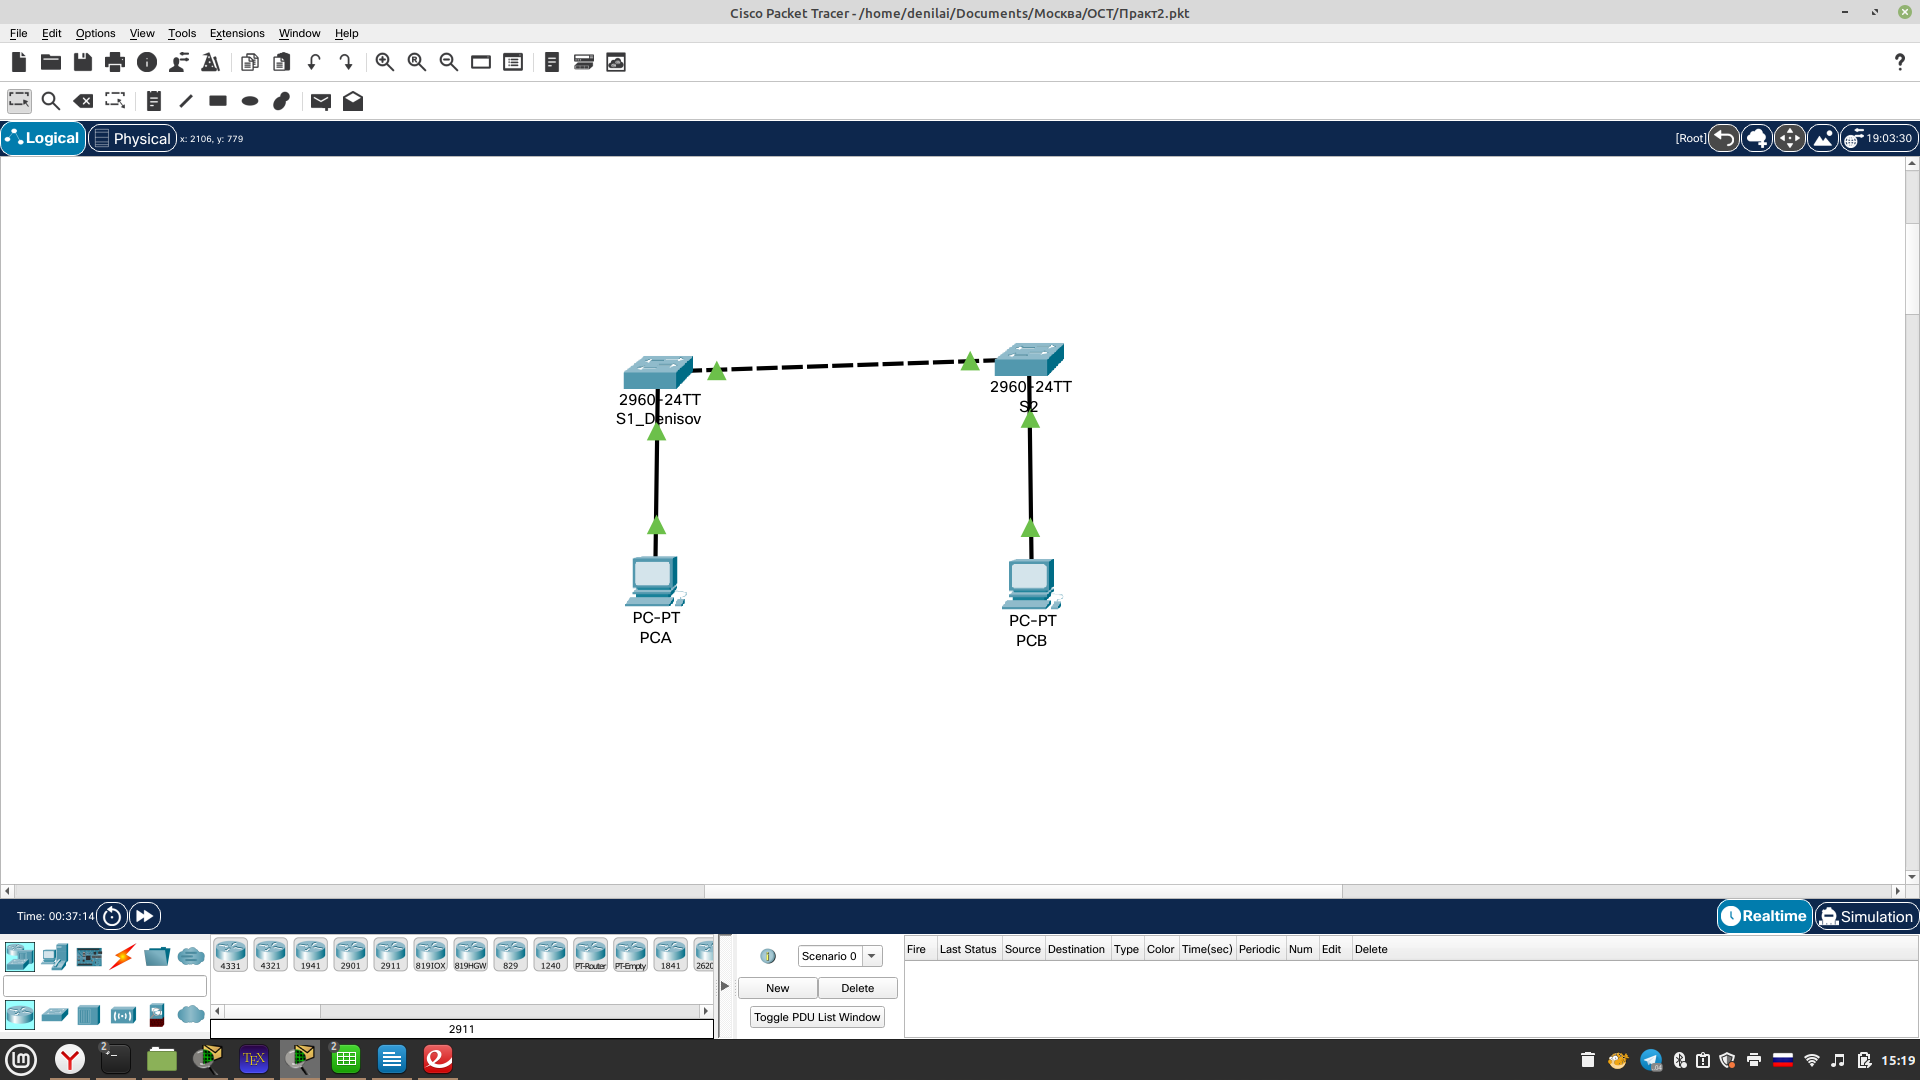
\includegraphics[width=0.7\linewidth]{images/topology}
	\caption{Топология сети}
	\label{fig:topology}
\end{figure}

\mypart{Настройка узлов ПК}
\step{Настройте статический IP-адрес на компьютерах}
Настроим статический IP-адрес на компьютерах в соответствии в заданием. Воспользуемся графическим интерфейсом \pt (см. рис. \ref{fig:ips}).

% TODO: \usepackage{graphicx} required
\begin{figure}[h!]
	\centering
	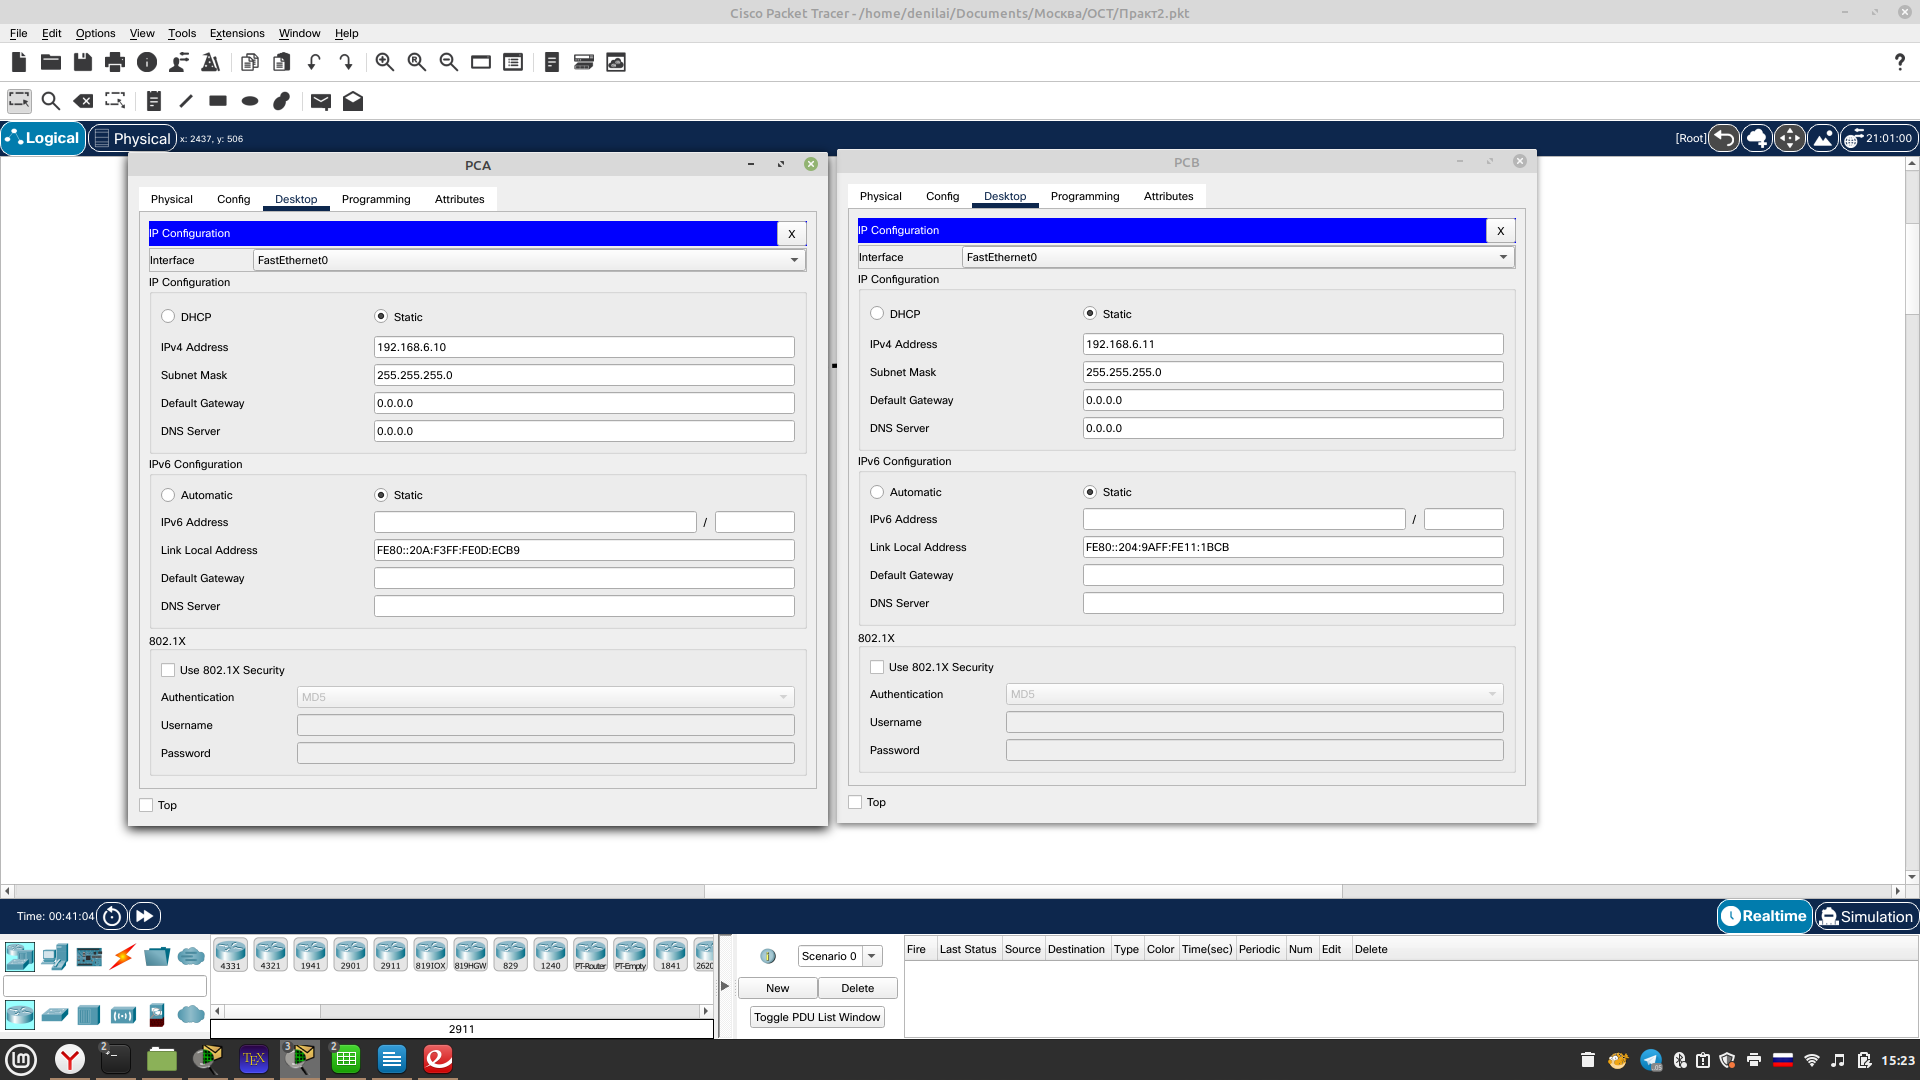
\includegraphics[width=0.7\linewidth]{images/IPs}
	\caption{Настройка IP-адресов}
	\label{fig:ips}
\end{figure}

\step {Проверьте настройки ПК и подключения}
Проверим конфигурацию компьютеров, выполнив команду 
\begin{lstlisting}
	ipconfig \all
\end{lstlisting}
Отправим эхо запрос по адресу 192.168.6.11, чтобы проверить возможность связи с компьютером PC-B. (см. рис. \ref{fig:ping-pc-b}).
% TODO: \usepackage{graphicx} required
\begin{figure}
	\centering
	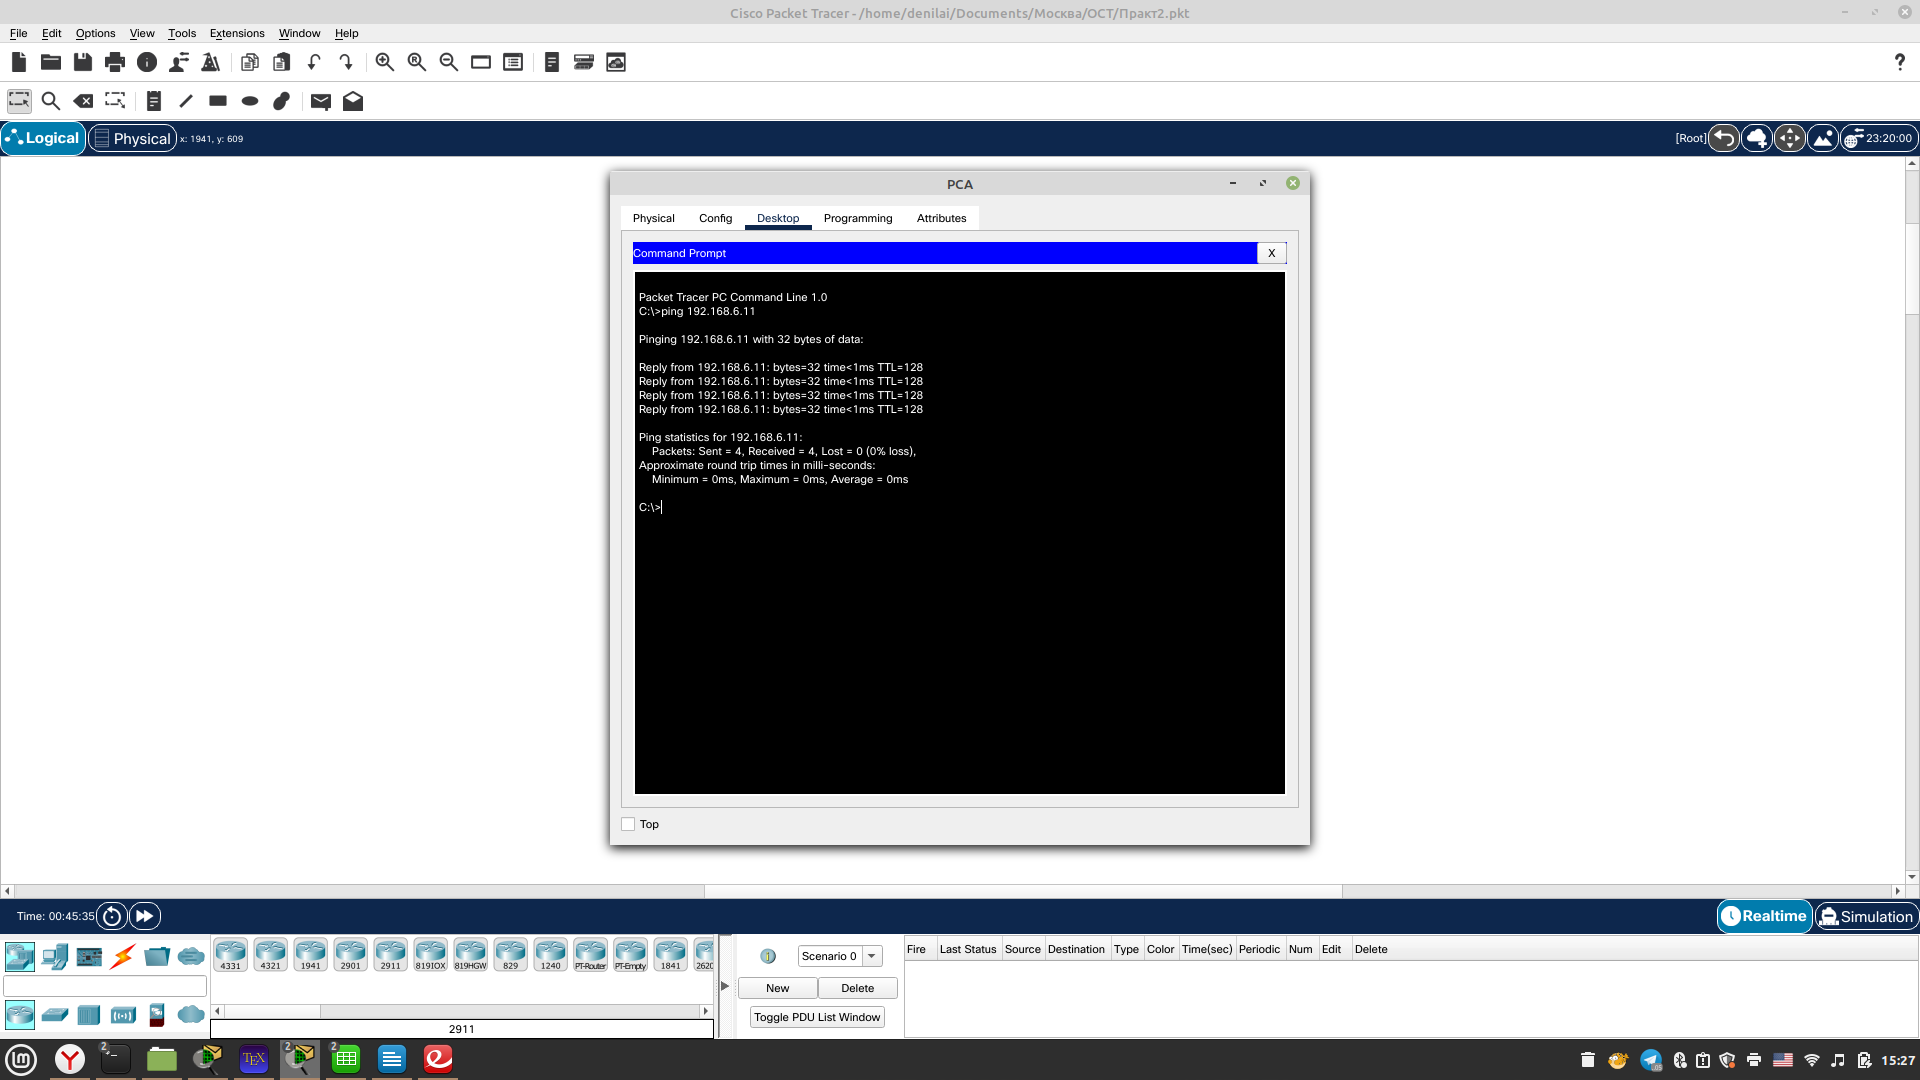
\includegraphics[width=0.7\linewidth]{images/ping-pc-b}
	\caption{Проверка соединения}
	\label{fig:ping-pc-b}
\end{figure}

\mypart{Базовая настройка и проверка настроек коммутатора}
\step{Подключитесь к коммутатору через консоль}
С графического интерфейса \pt получим доступ к  коммутатору через консоль.
\step{Войдите в привилегированный режим EXEC}
Перейдем в привилегированный режим EXEC, выполнив команду \textit{enable}.
\begin{lstlisting}
	Switch> enable
	Switch #
\end{lstlisting}

Приглашение в командной строке изменится с Switch> на Switch\#, что указывает на привилегированный режим EXEC.
\step{Войдите в режим глобальной конфигурации}
Для входа в режим конфигурации используем команду \textit{configuration terminal}.
\begin{lstlisting}
	Switch# configure terminal
	Enter configuration commands, one per line. End with CNTL/Z.
	Switch(config)#
\end{lstlisting}
\step{Присвойте коммутатору имя}
С помощью команды \textit{hostname} изменим имя коммутатора на S1\_Denisov.
\begin{lstlisting}
	Switch(config)# hostname S1
	S1_DENISOV(config)#
\end{lstlisting}
\step{Запретите попытки коммутатора преобразовывать неверные команды, как будто
	они являются именами узлов}
Отключим поиск в DNS, чтобы предотвратить попытки коммутатора преобразовывать введенные
команды таким образом, как будто они являются именами узлов.
\begin{lstlisting}
	S1_DENISOV(config)# no ip domain-lookup
	S1_DENISOV(config)#
\end{lstlisting}

\step{Введите локальные пароли}
\begin{lstlisting}
	S1_DENISOV(config)# enable secret class
	S1_DENISOV(config)# line con 0
	S1_DENISOV(config-line)# password cisco
	S1_DENISOV(config-line)# login
	S1_DENISOV(config-line)# exit
	S1_DENISOV(config)#
\end{lstlisting}
\step{Введите баннер MOTD (сообщение дня)}
\begin{lstlisting}
	S1_DENISOV(config)# banner motd "This is a secure system. Authorized Access Only!"
\end{lstlisting}
\step{Настройте IP-адрес интерфейса SVI}
Настроим SVI. Для этого перейдем в режим конфигурации интерфейса vlan1.
\begin{lstlisting}
	S1_DENISOV(config)#interface vlan 1 
	S1_DENISOV(config-if)#ip address 192.168.6.1 255.255.255.0   
\end{lstlisting}
\step{Сохраните конфигурацию}
	С помощью команды copy сохраним текущую конфигурацию в файл загрузочной конфигурации,
который хранится в NVRAM.
\begin{lstlisting}
	S1_DENISOV# copy running-config startup-config
	Destination filename [startup-config]? [Enter]
	Building configuration...
	[OK]
	S1_DENISOV#
\end{lstlisting}
\step{Отобразите текущую конфигурацию}
Команда \textit{show running-config} отображает всю текущую конфигурацию постранично
\begin{lstlisting}
Building configuration...

Current configuration : 1288 bytes
!
version 15.0
no service timestamps log datetime msec
no service timestamps debug datetime msec
no service password-encryption
!
hostname Switch
!
enable secret 5 $1$mERr$hx5rVt7rPNoS4wqbXKX7m0
!
!
!
no ip domain-lookup
!
!
!
spanning-tree mode pvst
spanning-tree extend system-id
!
interface FastEthernet0/1
!
interface FastEthernet0/2
!
interface FastEthernet0/3
!
interface FastEthernet0/4
!
interface FastEthernet0/5
!
interface FastEthernet0/6
!
interface FastEthernet0/7
!
interface FastEthernet0/8
!
interface FastEthernet0/9
!
interface FastEthernet0/10
!
interface FastEthernet0/11
!
interface FastEthernet0/12
!
interface FastEthernet0/13
!
interface FastEthernet0/14
!
interface FastEthernet0/15
!
interface FastEthernet0/16
!
interface FastEthernet0/17
!
interface FastEthernet0/18
!
interface FastEthernet0/19
!
interface FastEthernet0/20
!
interface FastEthernet0/21
!
interface FastEthernet0/22
!
interface FastEthernet0/23
!
interface FastEthernet0/24
!
interface GigabitEthernet0/1
!
interface GigabitEthernet0/2
!
interface Vlan1
ip address 192.168.6.1 255.255.255.0
!
banner motd ^CThis is a secure system. Authorized Access Only!^C
!
!
!
line con 0
password cisco
login
!
line vty 0 4
password cisco
login
transport input telnet
line vty 5 15
login
!
!
!
!
end
\end{lstlisting}
\step{Отобразите версию IOS и другую информацию о коммутаторе}
С помощью команды\textit{ show version} отобразим версию IOS коммутатора, а также другую полезную
информацию. Здесь для пролистывания отображаемых данных также используется клавиша пробела. (см. рис. \ref{fig:version-listitng}).
% TODO: \usepackage{graphicx} required
\begin{figure}[h!]
	\centering
	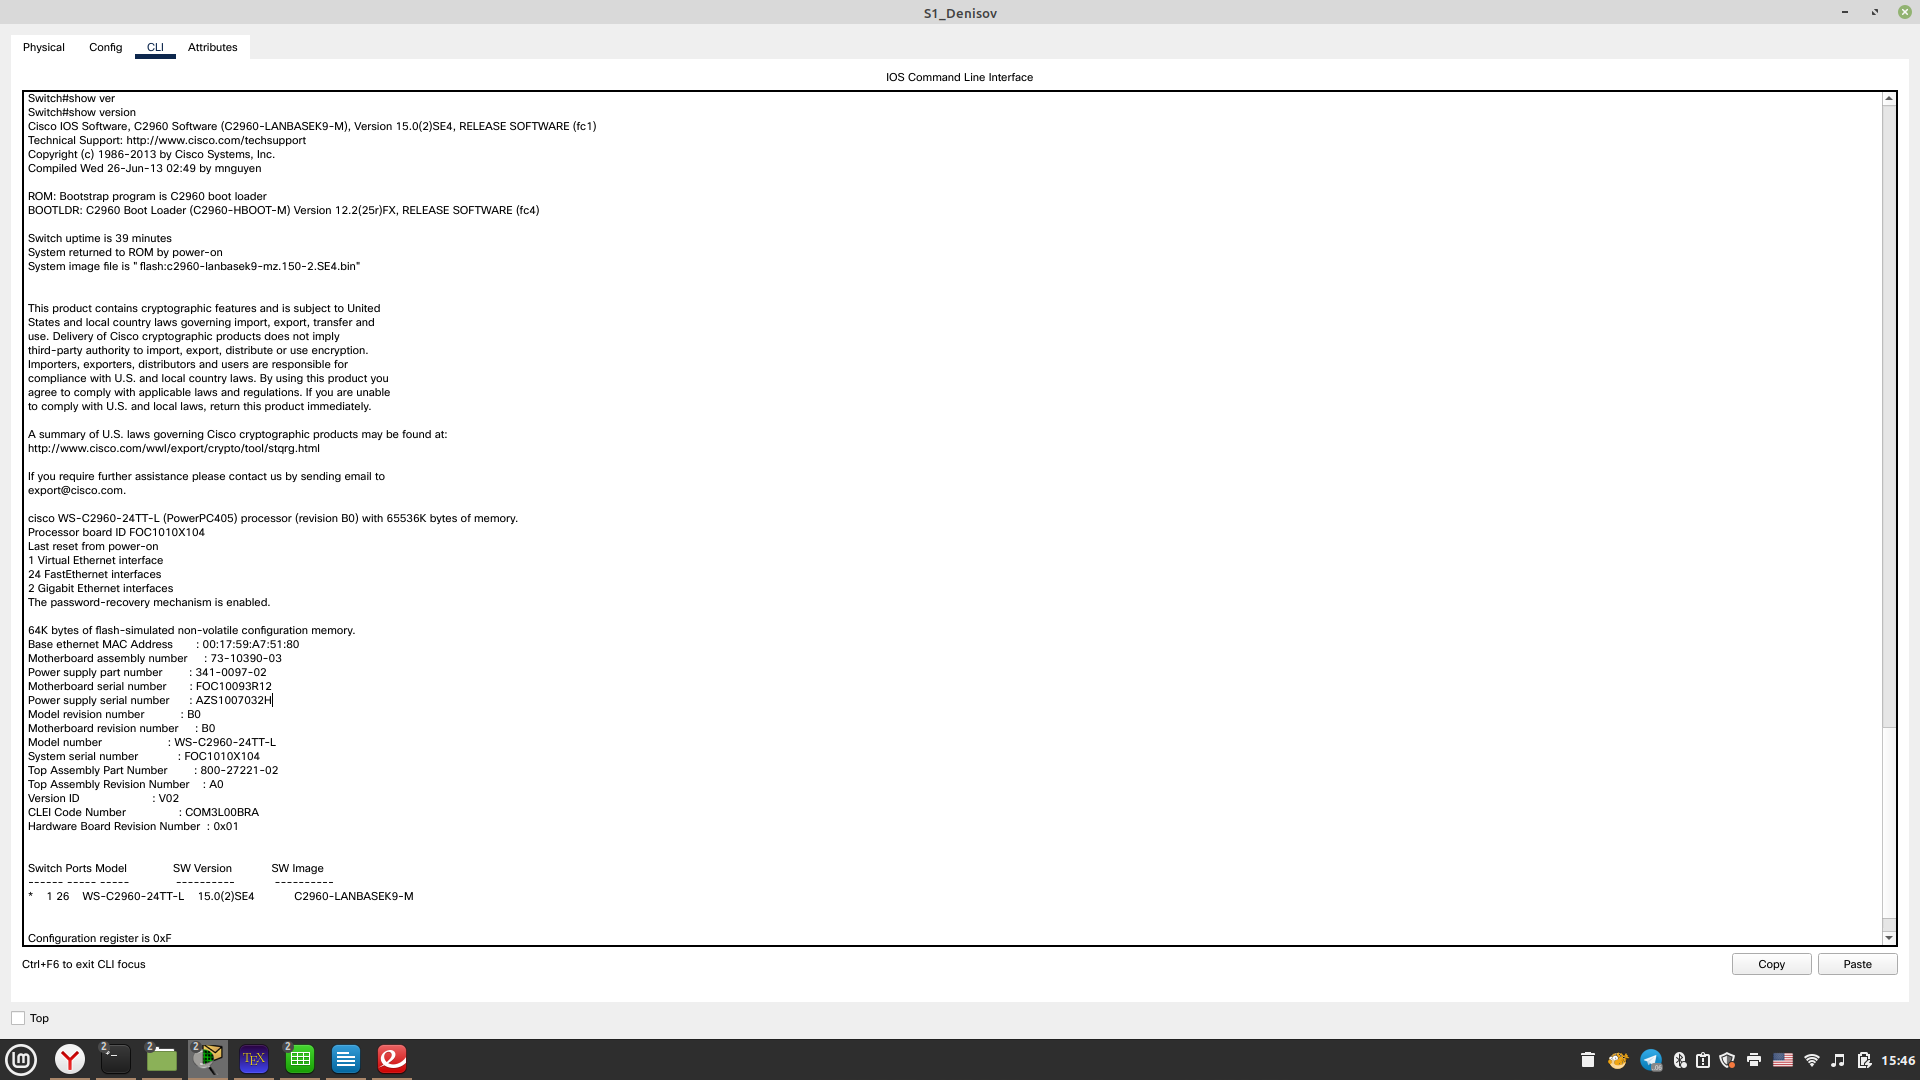
\includegraphics[width=0.7\linewidth]{images/version-listitng}
	\caption{Вывод команды show verison}
	\label{fig:version-listitng}
\end{figure}

\step{Отобразите состояние подключенных интерфейсов коммутатора}
Для проверки состояния подключенных интерфейсов используем команду \textit{show ip interface brief}. Для
пролистывания списка используйте клавишу пробела. (см. рис. \ref{fig:interface-listing} ).

% TODO: \usepackage{graphicx} required
\begin{figure}[h!]
	\centering
	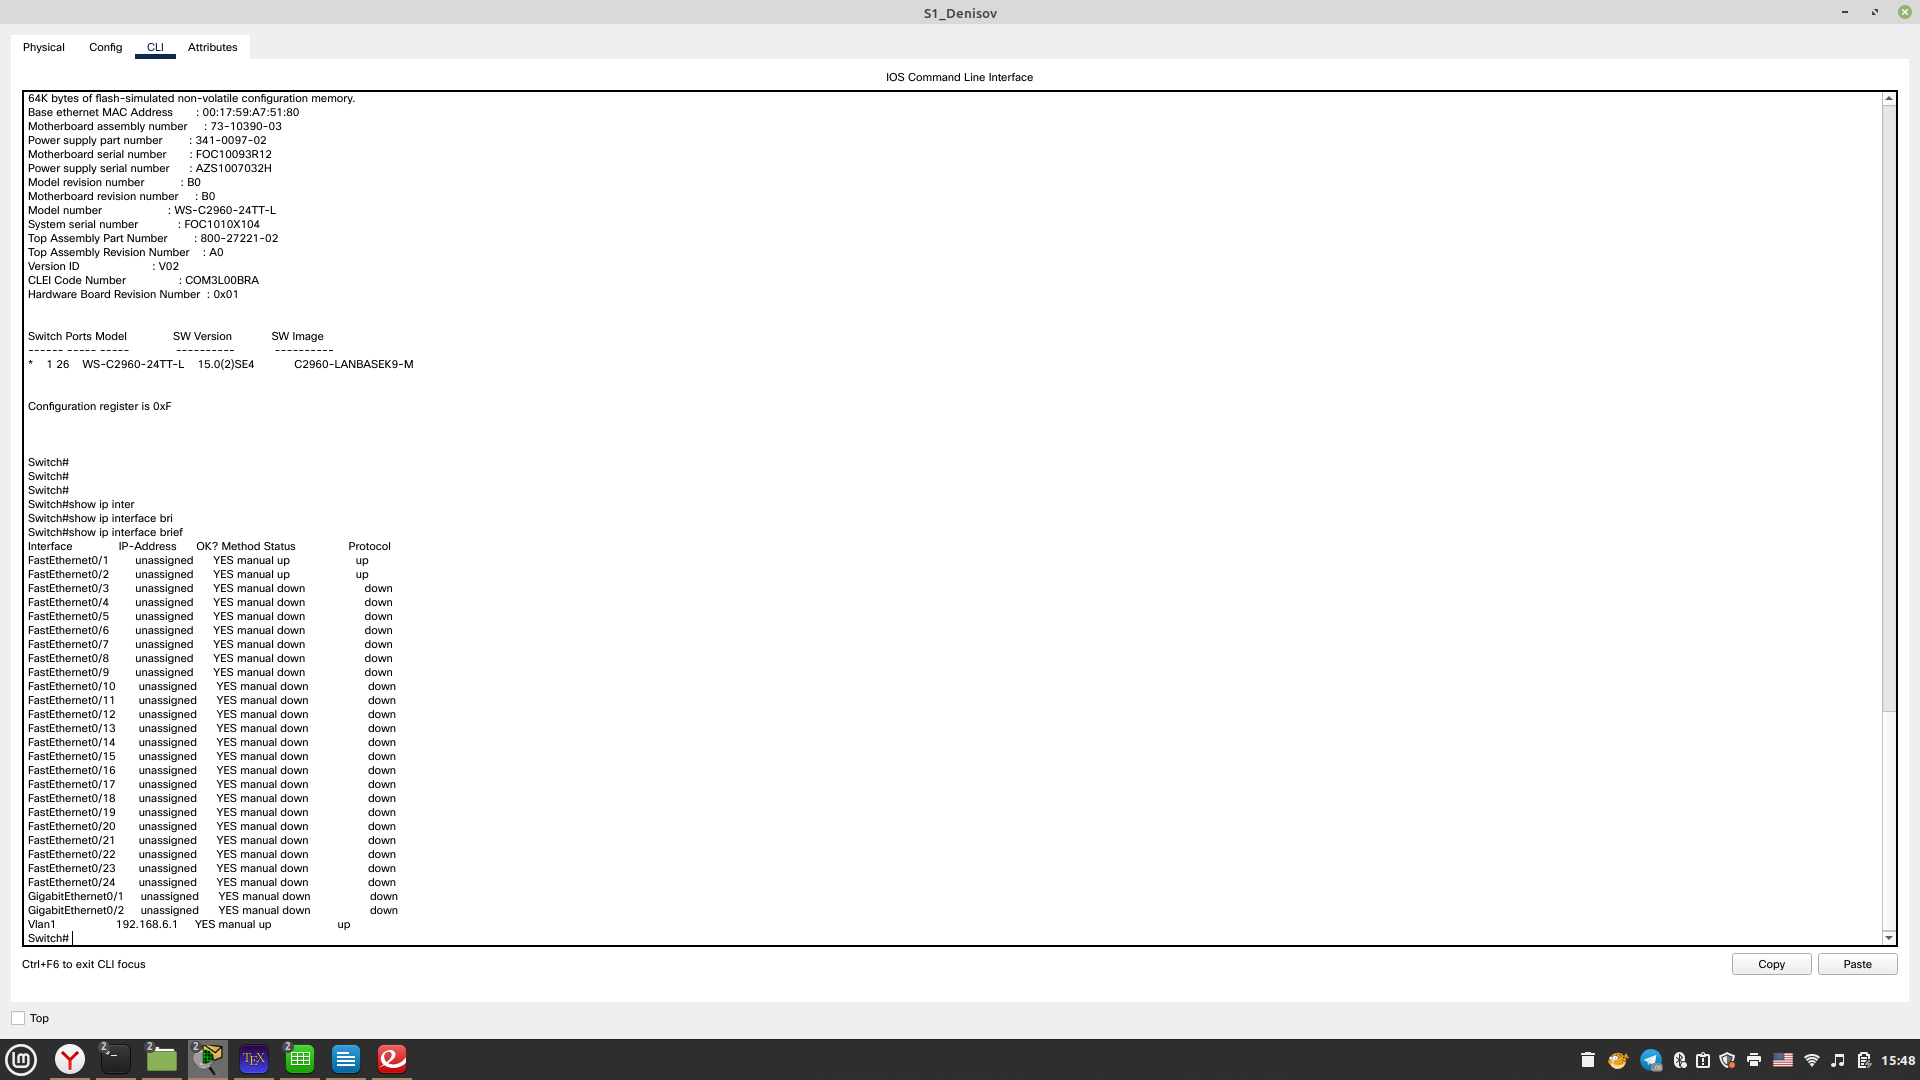
\includegraphics[width=0.7\linewidth]{images/interface-listing}
	\caption{Вывод команды show ip interface brief }
	\label{fig:interface-listing}
\end{figure}

\step{Подключитесь к коммутатору S1\_DENISOV по протоколу Telnet}
Подключимся к коммутатору S1\_DENISOV по протоколу Telnet (см. рис. \ref{fig:telnet-sw1}).
% TODO: \usepackage{graphicx} required
\begin{figure}[htpb]
	\centering
	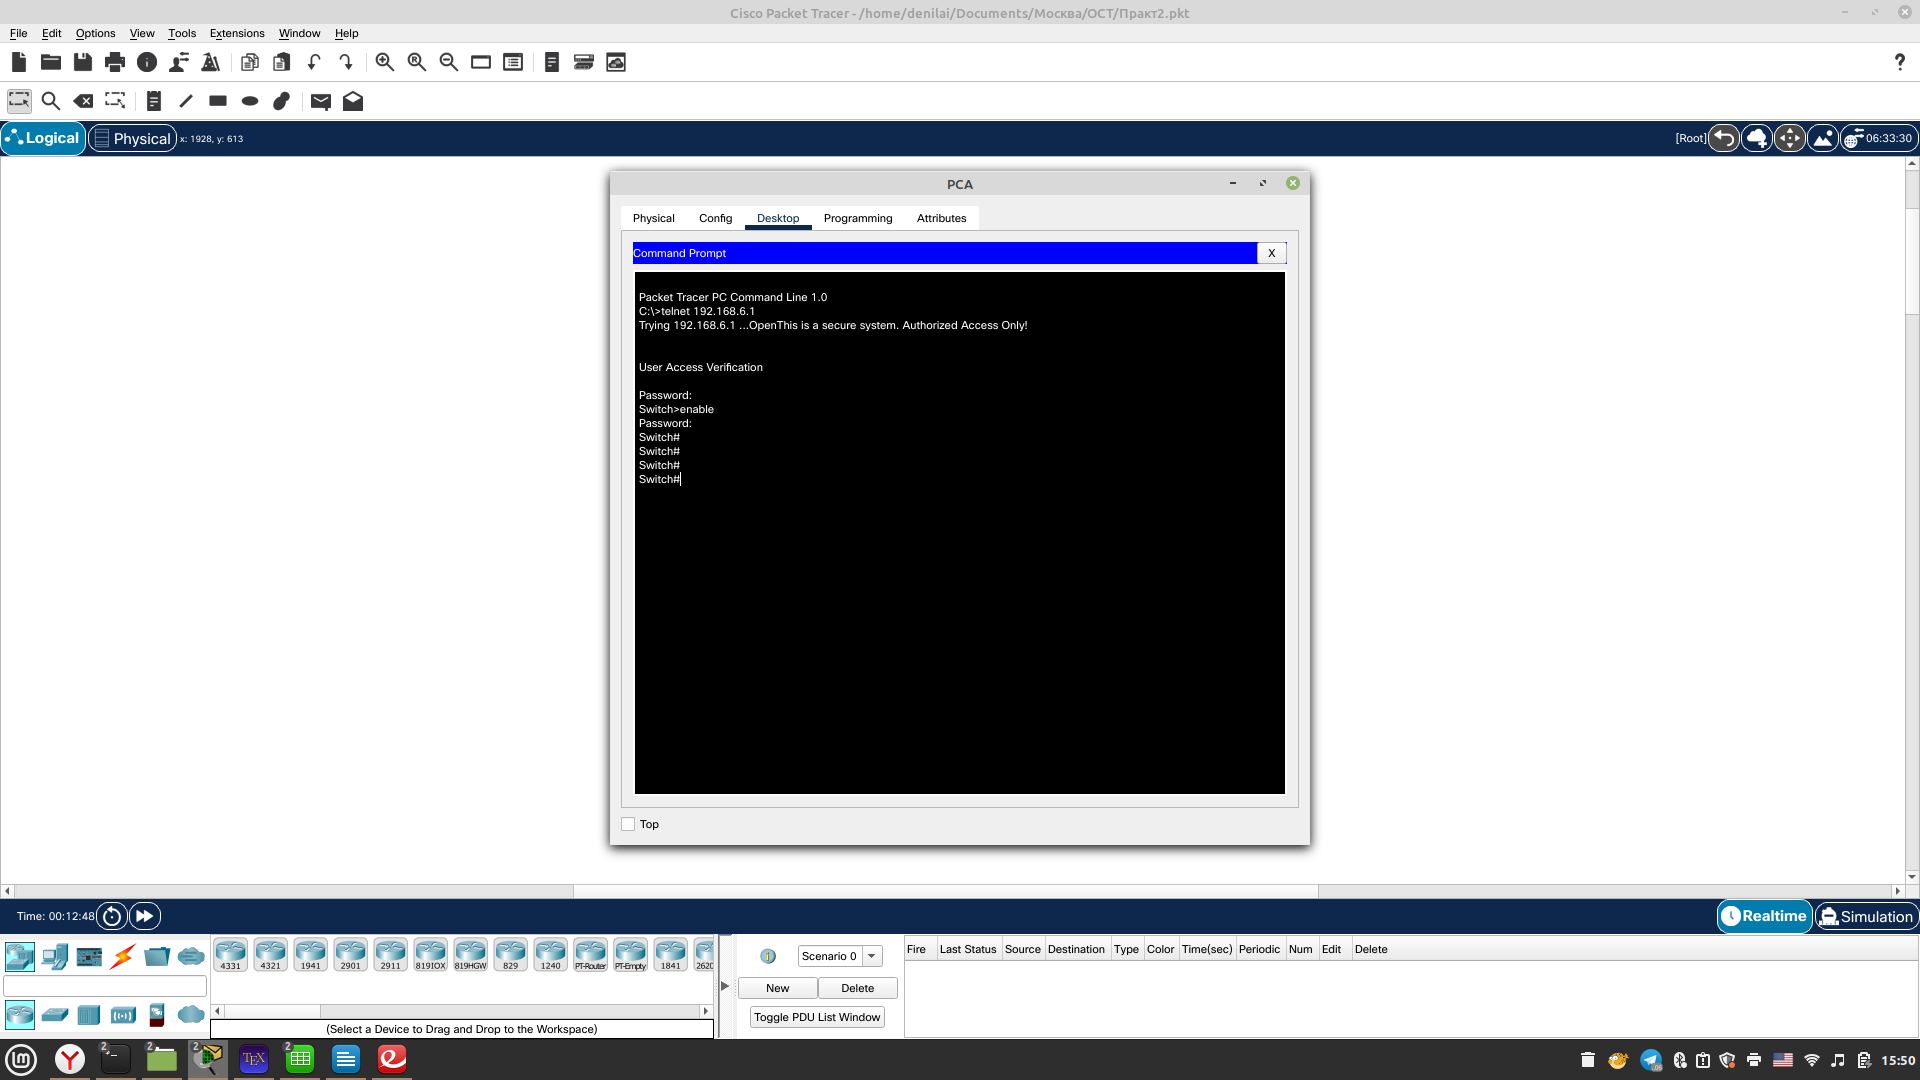
\includegraphics[width=0.7\linewidth]{images/telnet-sw1}
	\caption{Подключение к коммутатору по протоколу Telnet}
	\label{fig:telnet-sw1}
\end{figure}
\newpage
\step{Повторите шаги 1–13 для настройки коммутатора S2}
Выполним аналогичные шаги для коммутатора S2. Приведем его текущую конфигурацию.
\begin{lstlisting}
	Building configuration...
	
	Current configuration : 1288 bytes
	!
	version 15.0
	no service timestamps log datetime msec
	no service timestamps debug datetime msec
	no service password-encryption
	!
	hostname Switch
	!
	enable secret 5 $1$mERr$hx5rVt7rPNoS4wqbXKX7m0
	!
	!
	!
	no ip domain-lookup
	!
	!
	!
	spanning-tree mode pvst
	spanning-tree extend system-id
	!
	interface FastEthernet0/1
	!
	interface FastEthernet0/2
	!
	interface FastEthernet0/3
	!
	interface FastEthernet0/4
	!
	interface FastEthernet0/5
	!
	interface FastEthernet0/6
	!
	interface FastEthernet0/7
	!
	interface FastEthernet0/8
	!
	interface FastEthernet0/9
	!
	interface FastEthernet0/10
	!
	interface FastEthernet0/11
	!
	interface FastEthernet0/12
	!
	interface FastEthernet0/13
	!
	interface FastEthernet0/14
	!
	interface FastEthernet0/15
	!
	interface FastEthernet0/16
	!
	interface FastEthernet0/17
	!
	interface FastEthernet0/18
	!
	interface FastEthernet0/19
	!
	interface FastEthernet0/20
	!
	interface FastEthernet0/21
	!
	interface FastEthernet0/22
	!
	interface FastEthernet0/23
	!
	interface FastEthernet0/24
	!
	interface GigabitEthernet0/1
	!
	interface GigabitEthernet0/2
	!
	interface Vlan1
	ip address 192.168.6.2 255.255.255.0
	!
	banner motd ^CThis is a secure system. Authorized Access Only!^C
	!
	!
	!
	line con 0
	password cisco
	login
	!
	line vty 0 4
	password cisco
	login
	transport input telnet
	line vty 5 15
	login
	!
	!
	!
	!
	end
\end{lstlisting}
\step{Запишите состояние указанных ниже интерфейсов}

\begin{table}[h!]
	\begin{center}
		\caption{Состояние интерфейсов}
	\begin{tabular}{|c|c|c|c|c|}
		\hline
		& \multicolumn{2}{|c|}{S1\_DENISOV}  & \multicolumn{2}{c|}{S2}  \\
		\hline
		Интерфейс & Статус & Протокол & Статус & Протокол \\
		\hline
		FE0/1 & up & up & up & up \\
		FE0/2 &  up & up &  down &  down\\
		FE0/15 &  down &  down&   down &  down\\
		\hline
	\end{tabular}
	\label{tab:interface-status}
	\end{center}
\end{table}
Причина того, почему некоторые порты выключены в том, что все подключенные порты включены. Другие по умолчанию отключены. Vlan1 также отключена по умолчанию в \pt.

\end{document}

